\chapter{Class diagram of enumerator classes}
\label{app:uml}

\begin{figure}[H]
    \centering
    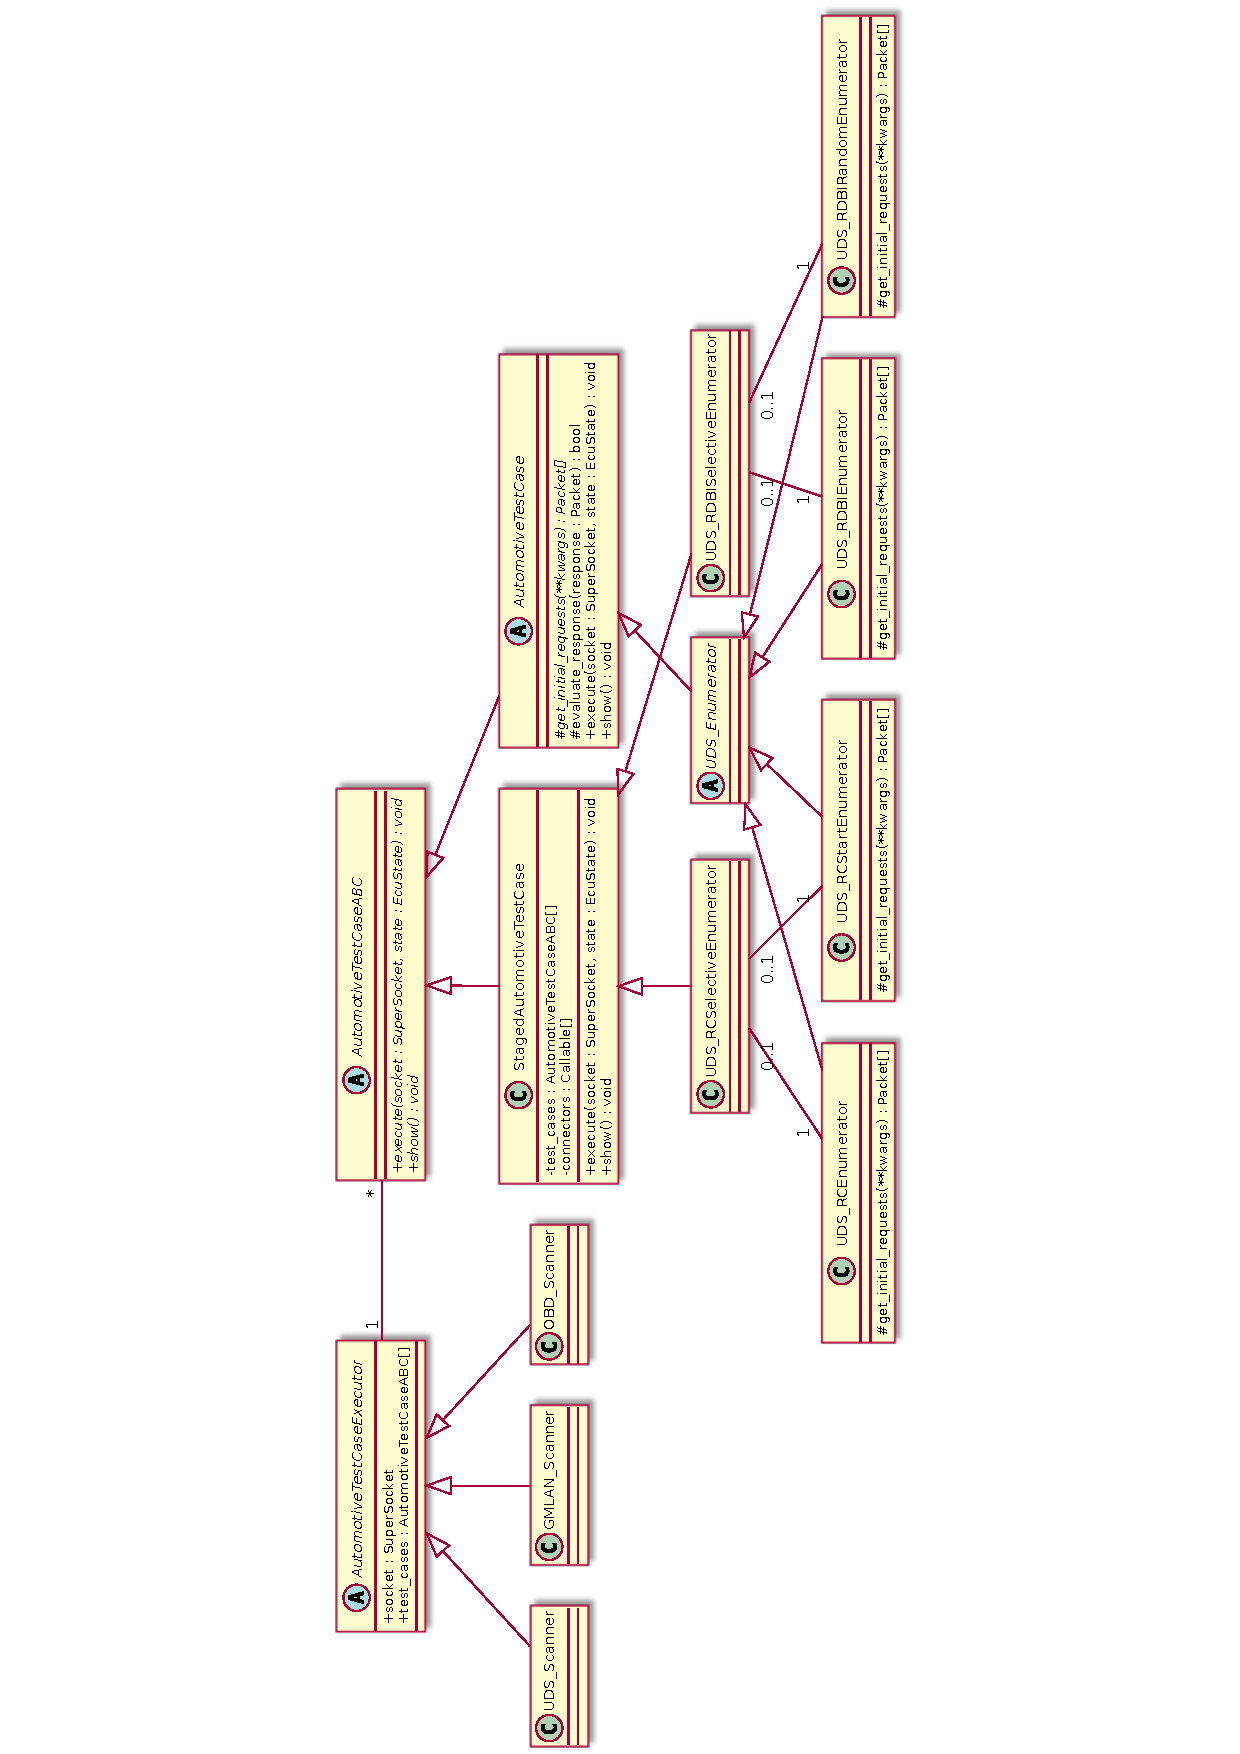
\includegraphics[height=0.9\textheight]{uml/overview}
\end{figure}

\chapter{Alternative versions of the RDBI implementation}

\section{First version of the random enumerator}
\label{app:random-not-compact}

\begin{minted}
[frame=single,
framerule=0pt,
framesep=2mm,
baselinestretch=1.2,
bgcolor=VeryLightGray,
fontsize=\footnotesize,
linenos]
{python}
def _get_initial_requests(self, **kwargs):
    samples_per_block = [
        1, 0, 0, 0, 29, 22, 19, 0, 11, 11, 13, 14, 31, 4, 26, 1,
        30, 4, 20, 5, 49, 54,
        9, 4, 10, 8, 0, 0, 6, 3, 1, 0, 11, 0, 1, 0, 4, 3, 0, 1, 9,
        9, 3, 1, 2, 0, 0, 3,
        4, 3, 0, 0, 8, 0, 0, 0, 0, 0, 0, 0, 0, 0, 0, 0, 35, 0, 2,
        1, 24, 19, 30, 28,
        16, 4, 6, 27, 41, 11, 6, 0, 0, 2, 0, 1, 0, 0, 1, 0, 3, 0,
        2, 1, 16, 0, 0, 0, 0,
        15, 20, 0, 6, 5, 5, 10, 0, 1, 10, 0, 4, 0, 0, 0, 0, 0, 0,
        0, 0, 0, 0, 0, 0, 0,
        0, 0, 3, 0, 0, 0, 7, 0, 0, 0, 0, 0, 1, 0, 15, 14, 27, 10,
        0, 0, 0, 0, 0, 0, 1,
        0, 9, 0, 2, 0, 2, 0, 0, 0, 0, 0, 0, 0, 0, 1, 0, 0, 0, 0, 0,
        0, 23, 15, 16, 16,
        2, 0, 0, 0, 3, 4, 2, 1, 1, 0, 0, 0, 0, 0, 0, 2, 0, 0, 0, 0,
        0, 0, 0, 0, 0, 0,
        0, 0, 0, 0, 0, 0, 0, 0, 0, 0, 0, 0, 0, 0, 0, 0, 0, 0, 0, 0,
        0, 0, 0, 0, 0, 0,
        0, 0, 0, 0, 0, 0, 0, 0, 3, 0, 0, 2, 0, 0, 1, 0, 8, 0, 0, 0,
        1, 0, 0, 0, 0, 0,
        0, 0, 25, 0, 0, 0, 7, 2, 0, 0, 0, 1, 0, 1, 1, 0, 1, 0, 0,
        0, 0, 0, 0, 0, 0, 0,
        0, 0, 1, 0, 0, 0, 0, 0, 0, 0, 0, 6, 0, 0, 2, 0, 0, 1, 0, 0,
        0, 0, 0, 0, 0, 0,
        0, 0, 0, 0, 0, 0, 0, 0, 0, 0, 1, 1, 0, 1, 2, 1, 1, 3, 0, 0,
        0, 3, 19, 0, 2, 2,
        0, 0, 4, 10, 3, 0, 8, 0, 0, 1, 3, 0, 1, 0, 0, 0, 0, 0, 0,
        0, 0, 0, 0, 0, 1, 0,
        0, 0, 0, 0, 0, 0, 0, 0, 0, 0, 0, 0, 0, 0, 0, 0, 0, 0, 0, 0,
        0, 0, 0, 0, 0, 0,
        0, 0, 0, 0, 0, 0, 0, 0, 0, 0, 0, 0, 0, 0, 0, 0, 0, 0, 0, 0,
        0, 0, 0, 0, 0, 0,
        0, 0, 0, 0, 0, 0, 0, 0, 0, 0, 0, 0, 0, 0, 0, 0, 0, 0, 0, 0,
        0, 0, 0, 0, 0, 0,
        0, 0, 0, 0, 0, 0, 0, 0, 0, 0, 0, 0, 0, 0, 0, 0, 0, 0, 0, 0,
        0, 0, 0, 0, 0, 0,
        0, 0, 0, 0, 0, 0, 0, 0, 0, 0, 0, 0, 0, 0, 0, 0, 0, 0, 0, 0,
        0, 0, 0, 0, 0, 0,
        0, 0, 0, 0, 0, 0, 0, 0, 0, 0, 0, 0, 0, 0, 0, 0, 0, 0, 0, 0,
        0, 0, 0, 0, 0, 0,
        0, 0, 0, 0, 0, 0, 0, 0, 0, 0, 0, 0, 0, 0, 0, 0, 0, 0, 0, 0,
        0, 0, 0, 0, 0, 0,
        0, 0, 0, 0, 0, 0, 0, 0, 1, 0, 0, 0, 0, 0, 0, 0, 0, 0, 0, 0,
        0, 0, 0, 0, 0, 0,
        0, 0, 0, 0, 0, 0, 0, 0, 0, 0, 0, 0, 0, 0, 0, 0, 0, 0, 0, 0,
        0, 0, 0, 0, 0, 0,
        0, 0, 0, 0, 0, 0, 0, 0, 0, 0, 0, 0, 0, 0, 0, 0, 0, 0, 0, 0,
        0, 0, 0, 0, 0, 0,
        0, 0, 0, 0, 0, 0, 0, 0, 0, 0, 0, 0, 0, 0, 0, 0, 0, 0, 0, 0,
        0, 0, 0, 0, 0, 0,
        0, 0, 0, 0, 0, 0, 0, 0, 0, 0, 0, 0, 0, 0, 0, 0, 0, 0, 0, 0,
        0, 0, 0, 0, 0, 0,
        0, 0, 0, 0, 0, 0, 0, 0, 0, 0, 0, 0, 0, 0, 0, 0, 0, 0, 0, 0,
        0, 0, 0, 0, 0, 0,
        0, 0, 0, 0, 0, 0, 0, 0, 0, 0, 0, 0, 1, 0, 0, 0, 0, 0, 0, 0,
        0, 0, 0, 0, 0, 0,
        0, 0, 0, 0, 0, 0, 0, 0, 0, 0, 0, 0, 0, 0, 0, 0, 0, 0, 0, 0,
        0, 0, 0, 0, 0, 0,
        0, 0, 0, 0, 0, 0, 0, 0, 0, 0, 0, 0, 0, 0, 0, 0, 0, 0, 0, 0,
        0, 0, 0, 0, 0, 0,
        0, 0, 0, 0, 0, 0, 0, 0, 0, 0, 0, 0, 0, 0, 0, 0, 0, 0, 0, 0,
        0, 0, 0, 0, 0, 0,
        0, 0, 0, 0, 0, 0, 0, 0, 0, 0, 0, 0, 0, 0, 0, 0, 0, 0, 0, 0,
        0, 0, 0, 0, 0, 0,
        0, 0, 0, 0, 0, 0, 0, 0, 0, 0, 6, 2, 0, 0, 0, 0, 0, 0, 0, 0,
        0, 0, 0, 0, 0, 0,
        0, 0, 0, 0, 0, 0, 0, 0, 0, 0, 0, 0, 0, 0, 0, 0, 0, 0, 0, 0,
        0, 0, 0, 0, 0, 0,
        0, 0, 0, 0, 0, 0, 0, 0, 0, 0, 0, 0, 0, 0, 0, 0, 0, 0, 0, 0,
        0, 0, 0, 0, 0, 1,
        4, 0, 0, 0, 0, 0, 0, 0, 0, 0, 0, 0, 0, 0, 0, 0, 0, 0, 0, 0,
        0, 0, 0, 0, 0, 0,
        0, 0, 0, 0, 0, 0, 0, 0, 0, 0, 0, 0, 0, 0, 0, 0, 0, 0, 0, 0,
        0, 0, 0, 0, 0, 0,
        0, 0, 0, 0, 4, 0, 3, 1, 0, 0, 0, 0, 12, 13, 34, 3, 0, 0, 0,
        0, 10, 0, 0, 0, 0,
        0, 0, 0, 0, 0, 0, 0, 0, 0, 0, 0, 0, 0, 0, 0, 0, 0, 0, 0, 0,
        0, 0, 0, 3, 0, 0,
        0, 0, 0, 0, 0, 0, 0, 0, 0, 23, 14, 15, 0, 0, 0, 0, 0, 0, 0,
        0, 0]


    to_scan = []
    block_size = UDS_RDBIRandomEnumerator.block_size
    for block_index, start in enumerate(range(0, 2 ** 16, block_size)):
        end = start + block_size
        count_samples = max(probabilities[block_index] * block_size, 1)
        to_scan += random.sample(range(start, end), count_samples)

    # Remaining code did not change
    # [...]
\end{minted}


\section{The RDBI connector using unofficial interfaces}
\label{app:unofficial-implementation}

\begin{minted}
    [frame=single,
    framerule=0pt,
    framesep=2mm,
    baselinestretch=1.2,
    bgcolor=VeryLightGray,
    fontsize=\footnotesize,
    linenos]
    {python}
@staticmethod
def __connector_random_to_sequential(rdbi_random, rdbi_sequential):
    prs_grouped_by_state = defaultdict(list)
    for r in rdbi_random.results_with_positive_response:
        prs_grouped_by_state[r.state].append(r.resp.dataIdentifier)

    block_size = UDS_RDBISelectiveEnumerator.block_size

    reqs_grouped_by_state = {}
    for state, ids in prs_grouped_by_state.items():
        scan_range = points_to_blocks(ids, block_size)
        req_ids = sorted(set(scan_range) - set(ids))
        reqs_grouped_by_state[state] = iter(
            (UDS() / UDS_RDBI(identifiers=[req_id]) for req_id in req_ids)
        )

    # By setting this, get_initial_requests of rdbi_sequential will never be called
    # as the requests per state are already set here.
    # Not intended by UDS Scanner developer
    rdbi_sequential._request_iterators = reqs_grouped_by_state

    # Do not return any configuration because it will not be used either way
    return {}
\end{minted}
